\section{Elements\index{Elements}}

The base for every Finite Elements computation is its mesh and the elements that are used within that mesh. The element types that can be used depend on the mesh, but also on the dimensionality of the problem (1D, 2D or 3D). In \akantu several isoparametric Langrangian element types are supported (and one serendipity element). Each of these types is discussed in some detail below, starting with the 1D-elements all the way to the 3D-elements. More detailed information (shape function, location of Gaussian quadrature points, and so on) can be found in Appendix~\ref{app:elements}. 

%%%%%%%%%% 1D %%%%%%%%%
\subsection{Isoparametric Elements\index{Elements!Isoparametric}}

\subsubsection*{1D\index{Elements!1D}}

In \akantu there are two types of isoparametric elements defined in 1D. These element types are called \code{\_segment\_2} and \code{\_segment\_3} and are depicted schematically in Figure~\ref{fig:elements:1D}. Some of the basic properties of these elements are listed in Table~\ref{tab:elements:1D}.

\begin{figure}[!htb]
\begin{center}
\begin{tabular}{m{0.3\textwidth}m{0.1\textwidth}m{0.3\textwidth}}
\subfloat[\code{\_segment\_2}]{
  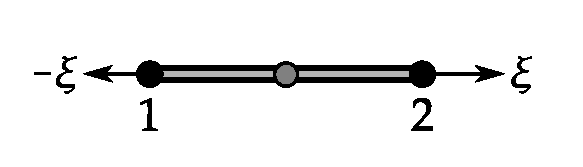
\includegraphics[width=0.3\textwidth]{figures/elements/segment_2}
  \label{fig:elements:segment2}
} & &
\subfloat[\code{\_segment\_3}]{
  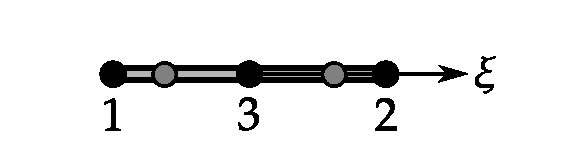
\includegraphics[width=0.3\textwidth]{figures/elements/segment_3}
  \label{fig:elements:segment3}
} 
\end{tabular}
\end{center}
\caption{Schematic overview of the two 1D element types in \akantu. In each element the node numbering as used in \akantu is indicated and also the quadrature points are highlighted (gray circles).}
\label{fig:elements:1D}
\end{figure}

\begin{table}[!htb]
\begin{center}
\begin{tabular}{l||c|c|c}
Element type & Order & \# nodes & \# quad. points \\
\hline
\code{\_segment\_2} & linear & 2 & 1 \\
\code{\_segment\_3} & quadratic & 3 & 2 \\
\end{tabular}
\end{center}
\caption{Some basic properties of the two 1D isoparametric elements in \akantu.}
\label{tab:elements:1D}
\end{table}

%%%%%%%%%% 2D %%%%%%%%%
\subsubsection*{2D\index{Elements!2D}}

In \akantu there are four types of isoparametric elements defined in 2D. These element types are called \code{\_triangle\_3}, \code{\_triangle\_6}, \code{\_quadrangle\_4} and \code{\_quadrangle\_8} and all of them are depicted in Figure~\ref{fig:elements:2D}. As with the 1D elements, some of the most basic properties of these elements are listed in Table~\ref{tab:elements:2D}. It is important to note that the first element is linear, the next two quadratic and the last one cubic. Furthermore, the last element type (\code{\_quadrangle\_8}) is not a Langrangian but a serendipity element.

\begin{figure}[!htb]
\begin{center}
\begin{tabular}{m{0.3\textwidth}m{0.1\textwidth}m{0.3\textwidth}}
\subfloat[\code{\_triangle\_3}]{
  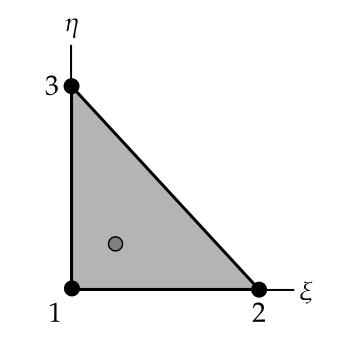
\includegraphics[width=0.3\textwidth]{figures/elements/triangle_3}
  \label{fig:elements:triangle3}
} & &
\subfloat[\code{\_triangle\_6}]{
  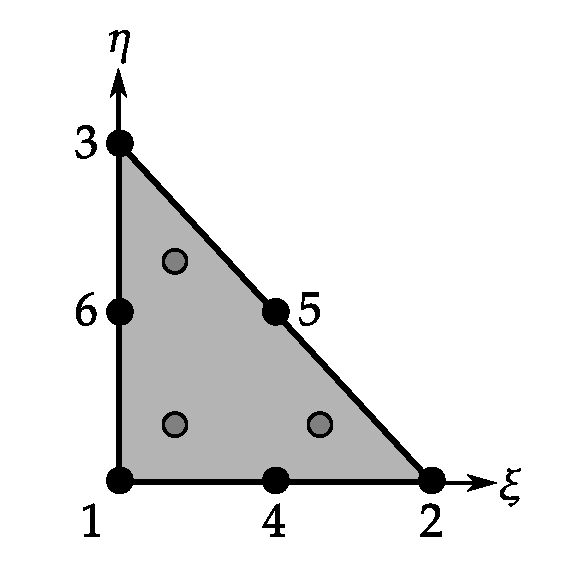
\includegraphics[width=0.3\textwidth]{figures/elements/triangle_6}
  \label{fig:elements:triangle6}
} \\
\subfloat[\code{\_quadrangle\_4}]{
  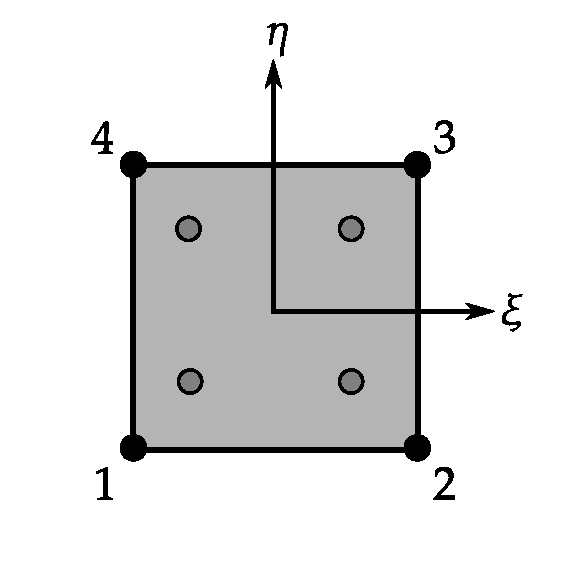
\includegraphics[width=0.3\textwidth]{figures/elements/quadrangle_4}
  \label{fig:elements:quadrangle4}
} & &
\subfloat[\code{\_quadrangle\_8}]{
  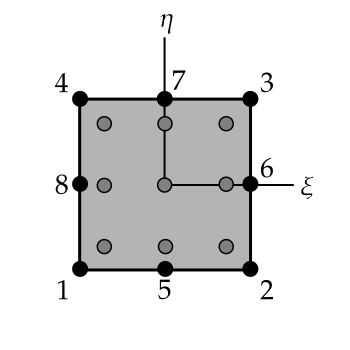
\includegraphics[width=0.3\textwidth]{figures/elements/quadrangle_8}
  \label{fig:elements:quadrangle8}
} 
\end{tabular}
\end{center}
\caption{Schematic overview of the four 2D element types in \akantu. In each element the node numbering as used in \akantu is indicated and also the quadrature points are highlighted (gray circles).}
\label{fig:elements:2D}
\end{figure}

\begin{table}[!htb]
\begin{center}
\begin{tabular}{l||c|c|c}
Element type & Order & \# nodes & \# quad. points \\
\hline
\code{\_triangle\_3} & linear & 3 & 1 \\
\code{\_triangle\_6} & quadratic & 6 & 3 \\
\hline
\code{\_quadrangle\_4} & quadratic & 4 & 4 \\
\code{\_quadrangle\_8} & cubic & 8 & 9 \\
\end{tabular}
\end{center}
\caption{Some basic properties of the four 2D isoparametric elements in \akantu.}
\label{tab:elements:2D}
\end{table}

%%%%%%%%%% 3D %%%%%%%%%
\subsubsection*{3D\index{Elements!3D}}

In \akantu there are three types of isoparametric elements defined in 3D. These element types are called \code{\_tetrahedron\_4}, \code{\_tetrahedron\_10} and \code{\_hexahedron\_8} and all of them are depicted schematically in Figure~\ref{fig:elements:3D}. As with the 1D and 2D elements some of the most basic properties of these elements are listed in Table~\ref{tab:elements:3D}.

\begin{figure}[!htb]
\begin{center}
\begin{tabular}{m{0.3\textwidth}m{0.3\textwidth}m{0.3\textwidth}}
\subfloat[\code{\_tetrahedron\_4}]{
  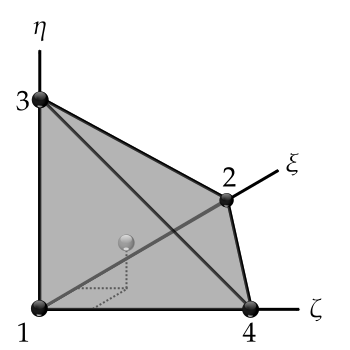
\includegraphics[width=0.3\textwidth]{figures/elements/tetrahedron_4}
  \label{fig:elements:tetrahedron4}
} &
\subfloat[\code{\_tetrahedron\_10}]{
  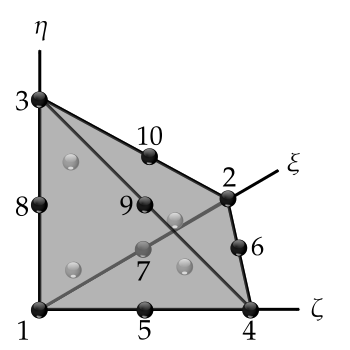
\includegraphics[width=0.3\textwidth]{figures/elements/tetrahedron_10}
  \label{fig:elements:tetrahedron10}
} &
\subfloat[\code{\_hexahedron\_8}]{
  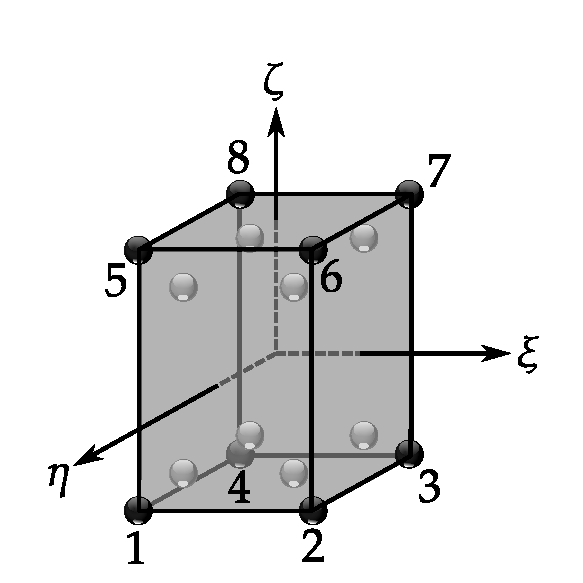
\includegraphics[width=0.3\textwidth]{figures/elements/hexahedron_8}
  \label{fig:elements:hexahedron8}
} 
\end{tabular}
\caption{Schematic overview of the three 3D element types in \akantu. In each element the node numbering as used in \akantu is indicated and also the quadrature points are highlighted (gray spheres).}
\label{fig:elements:3D}
\end{center}
\end{figure}

\begin{table}[!htb]
\begin{center}
\begin{tabular}{l||c|c|c}
Element type & Order & \# nodes & \# quad. points  \\
\hline
\code{\_tetrahedron\_4} & linear & 4 & 1  \\
\code{\_tetrahedron\_10} & quadratic & 10 & 4  \\
\hline
\code{\_hexahedron\_8} & cubic & 8 & 8  \\
\end{tabular}
\end{center}
\caption{Some basic properties of the three 3D isoparametric elements in \akantu.}
\label{tab:elements:3D}
\end{table}


%%%%%%%%%% STRUCTURAL ELEMENTS %%%%%%%%%

\subsection{Structural elements\index{Elements!Structural}}

\subsubsection*{Bernoulli beam elements\index{Elements!Bernoulli}}
These elements allow to compute the displacements and rotations of structures constituted by Bernoulli beams. \akantu defines them for both 2D and 3D problems in the element types \code{\_bernoulli\_beam\_2} and \code{\_bernoulli\_beam\_3}. A schematic depiction of a beam element is shown in Figure~\ref{fig:elements:bernoulli} and some of its properties are listed in Table~\ref{tab:elements:bernoulli}.

\note{Beam elements are of mixed order: the axial displacement is linearly interpolated while transverse displacements and rotations use cubic shape functions.}

\begin{figure}[htb]
  \centering
  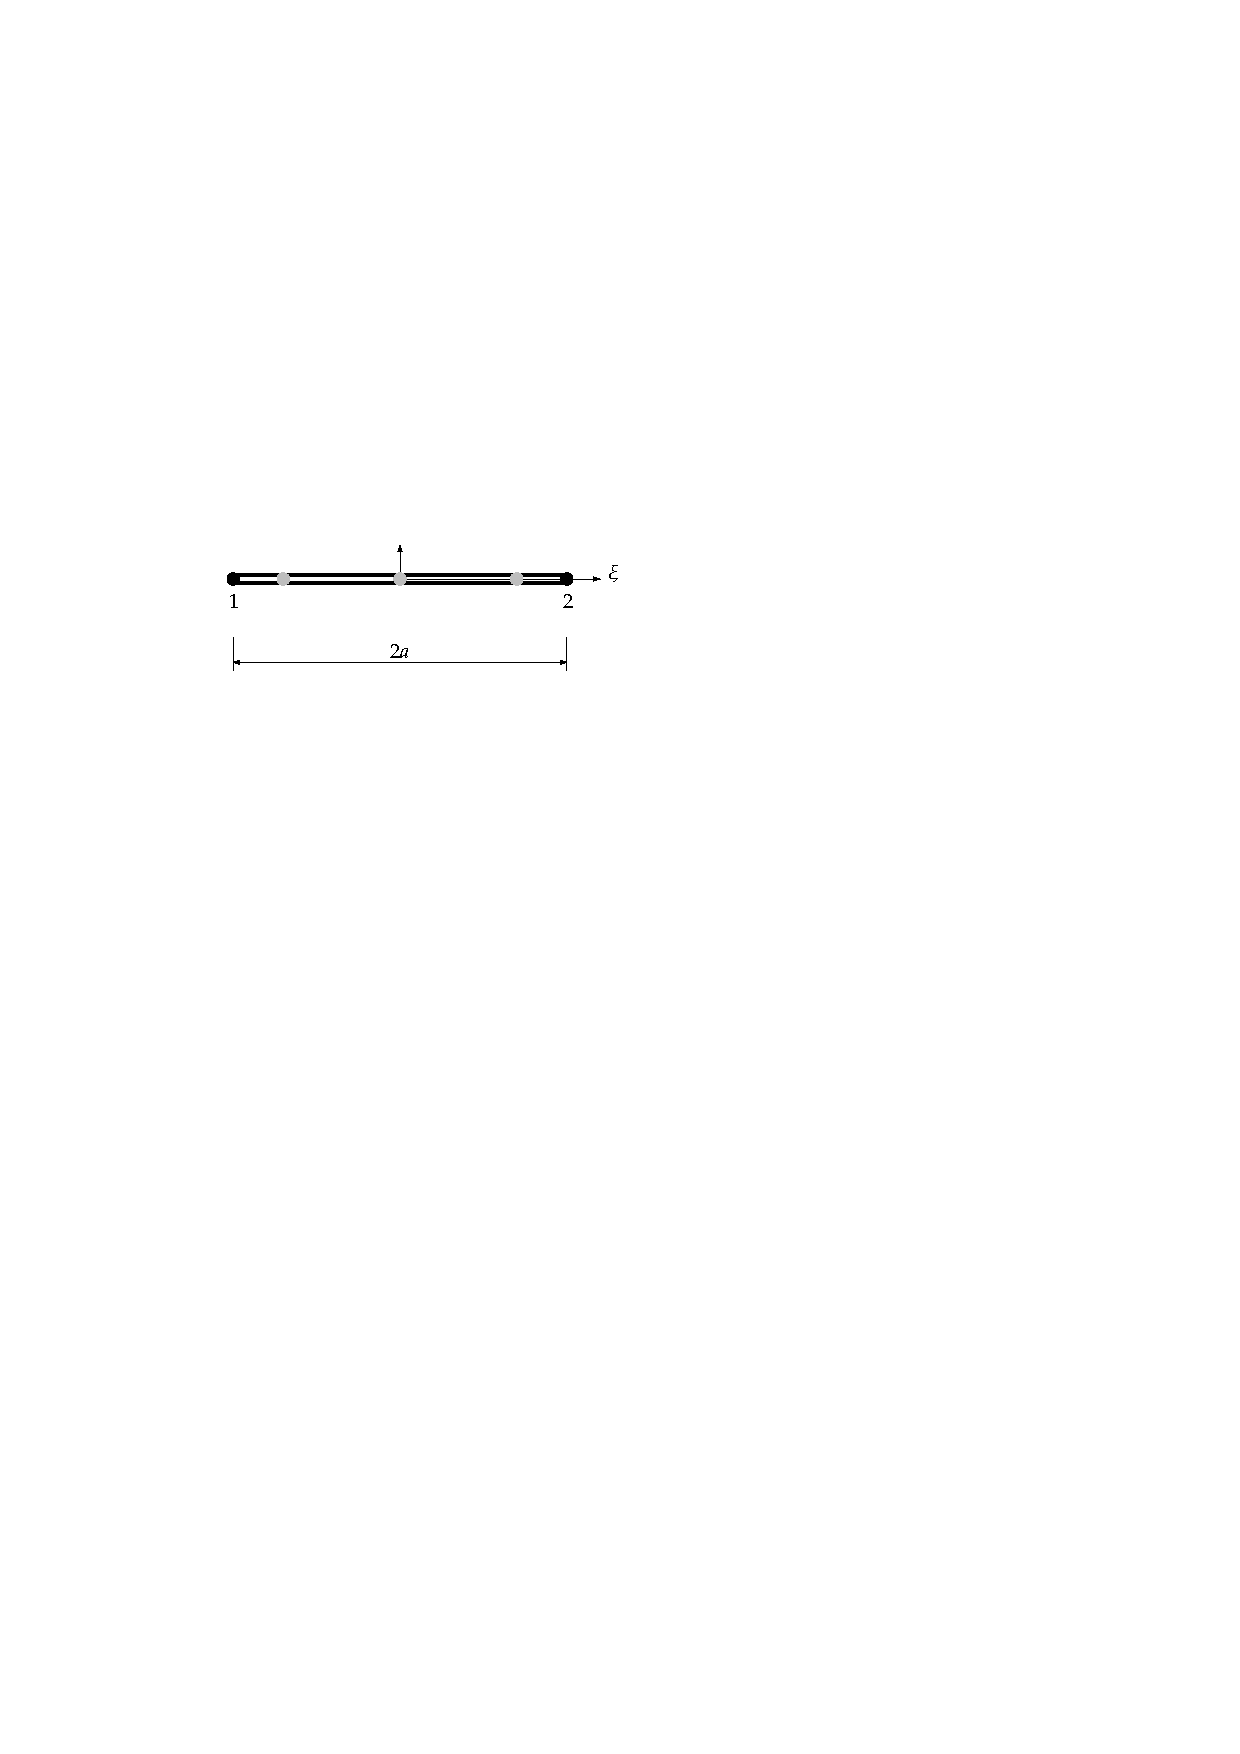
\includegraphics[width=0.3\textwidth]{figures/elements/bernoulli_2}
  \caption{Schematic depiction of a Bernoulli beam element (applies to 2D and 3D) in \akantu. The node numbering as used in \akantu is indicated and also the quadrature points are highlighted (gray circles).}
  \label{fig:elements:bernoulli}
\end{figure}
\begin{table}[htb]
  \centering
  \begin{tabular}{c||c|c|c|c}
    Element type &\#nodes &\#quad. points & \#dimensions & \#d.o.f.\\\hline\hline
    \code{\_bernoulli\_beam\_2} & 2&3 &2 &4\\\hline
    \code{\_bernoulli\_beam\_3} & 2&3 &3 &6
  \end{tabular}
  \caption{Some basic properties of \akantu's beam elements}
  \label{tab:elements:bernoulli}
\end{table}



%%% Local Variables:
%%% mode: latex
%%% TeX-master: "manual"
%%% End:


